%% Supplementary Information
%% What would make biodiversity offset markets work across all ecosystem types?
%% José Luis Reséndiz

\documentclass[pdflatex,sn-nature,oneside]{sn-jnl}

\usepackage{graphicx}
\usepackage{amsmath,amssymb}
\usepackage{booktabs}
\usepackage{xcolor}
\usepackage{hyperref}

\raggedbottom

\begin{document}

\title{Supplementary Information: What would make biodiversity offset markets work
       across all ecosystem types?}

\author*[1]{\fnm{José Luis} \sur{Reséndiz}}\email{jose.resendiz@smithschool.ox.ac.uk}

\affil*[1]{\orgdiv{Smith School of Enterprise and the Environment},
           \orgname{University of Oxford},
           \orgaddress{\city{Oxford}, \postcode{OX1 3QY}, \country{UK}}}

\maketitle


% ─────────────────────────────────────────────────────────────────────────────
% SUPPLEMENTARY NOTE 1
% ─────────────────────────────────────────────────────────────────────────────

\section*{Supplementary Note 1: Theoretical Foundations and Robustness}

\subsection*{1.1 Relationship to the market ecology framework}

Our theoretical framework originates in Farmer's~\cite{Farmer2002} demonstration that, under no density dependence, the wealth dynamics of competing trading strategies reduce to generalised Lotka-Volterra (GLV) equations: each strategy is treated as a biological species whose ``population'' (aggregate market share) grows or declines according to its profitability and its competitive interactions with other strategies. Scholl, Calinescu, and Farmer~\cite{SchollCalinescuFarmer2021} extended this insight to a calibrated agent-based model (ABM), and showed that the \emph{ecological community matrix} (computed numerically from the ABM via finite-difference perturbation of each species' population) captures the qualitative competitive structure: which strategies dominate, which are excluded, and which coexist.

We apply this framework to biodiversity credit markets, treating four behavioural strategies (cost-minimising compliance, mean-reversion intermediation, thin-market procurement, cost-floor supply) as ecological species competing for a finite pool of credit transactions. Three features of the NSW market support the GLV reduction. Compliance demand is exogenous and mandatory: developers must retire credits to satisfy planning conditions, so participation is regulatorily set rather than profit-driven. The market is segmented by vegetation formation, with 15 distinct sub-markets (corresponding to the 15 Keith vegetation formations in NSW), each with its own supply--demand balance. Trading is infrequent (approximately 12 ecosystem credit transactions per month across the scheme), so the wealth dynamics $W_i(t+1)=(1+f\pi_i(t))W_i(t)$ run on a slower timescale than the price-clearing process. Each of the three conditions Farmer (2002) requires for the GLV reduction is therefore satisfied directly: price formation per transaction is local under the discrete matching rule; compliance demand is exogenously partitioned across formations by IBRA subregion, mediating cross-formation interaction through within-formation substitution; and reinvestment timescales are slow relative to price formation.

The GLV provides numerically computed competitive-exclusion thresholds, irreversibility boundaries, and parameter sensitivity (computed by linear sweep over interaction multipliers and ODE re-integration; see \texttt{src/model/glv\_formation.py}). The ABM (252 real OTGs in 15 formations, with geographic demand concentration via IBRA subregions and stochastic bidding) provides Monte Carlo realism and confidence intervals. The ABM scenario ranking is Bypass Reduction $>$ Procurement Flexibility $>$ Rarity Multiplier $\geq$ Baseline $>$ Price Floor $>$ BCT Precision Mandate, and the GLV reproduces the same ordering. GLV policy multipliers (procurement-flexibility $\alpha$ multiplier $0.60$, bypass-reduction $r$ multiplier $1.20$; \texttt{src/model/glv\_formation.py}) are calibrated to the ABM's policy responses; cross-model agreement is established at the level of \emph{baseline} interaction coefficients via the species-level community-matrix Spearman $\rho = 0.689$ described below. The 15$\times$15 formation-level interaction matrix is derived from the GLV's analytical Jacobian.

Following Scholl et al.'s methodology, we compute the 4$\times$4 species-level community matrix numerically from the ABM via finite-difference perturbation of each species' population (20\% perturbation, 20 Monte Carlo seeds per configuration). The Spearman rank correlation between the off-diagonal elements of the ABM-derived community matrix and the GLV $\boldsymbol\alpha$ is $\rho = 0.689$ ($p < 10^{-30}$), confirming that the GLV captures the species-level competitive structure of the ABM. The dominant formation in the calibrated ABM is Grassy Woodlands; the GLV's $K$-budget weighting ranks Saline Wetlands first when BCT budget corrections are not applied, illustrating that BCT-budget allocation is what shifts thin-market formations into viability. Under its baseline parametrisation the GLV identifies five formations at the exclusion threshold (Grasslands, Rainforests, Saline Wetlands, Arid Shrublands (Acacia sub-formation), and Heathlands); the calibrated ABM, with its BCT budget correction (AUD\,326,389 per agent per month, derived from IPART 2024--25 data), retains four of the five at sub-functional-coverage levels and predicts a single market extinction (Arid Shrublands (Acacia sub-formation)). Eigenvalue analysis of the surviving-species Jacobian confirms local stability of the equilibrium.


\subsection*{1.2 Demand function derivations}

Each agent type's demand (or supply) function is derived from a well-defined optimisation problem, following the theoretical structure of Scholl et al.~\cite{SchollCalinescuFarmer2021}. We summarise each derivation below.

\paragraph{Compliance buyer.}
Compliance buyers solve a cost minimisation problem subject to a regulatory constraint:
\begin{align}
    \min_{q} \quad & q \cdot p \notag \\
    \text{s.t.} \quad & q \geq \text{obligation} \notag \\
    & q \cdot p \leq W \cdot f \label{eq:compliance}
\end{align}
where $p$ is the credit price, $W$ is the developer's budget, and $f$ is the fraction of budget available for offsets. This is \emph{not} a utility maximisation problem: compliance buyers are cost minimisers with a hard regulatory constraint. The resulting demand is a smoothed step function:
\begin{equation}
    z(p) = \text{obligation} \cdot \sigma(\text{threshold} - p) \cdot \min\!\bigl(1,\, W f / p\bigr)
\end{equation}
where $\sigma(\cdot)$ is the logistic function and ``threshold'' is the price above which the developer pays into the Biodiversity Conservation Fund instead of purchasing credits on the open market. Properties: $z(p) > 0$ for all $p < \text{threshold}$ (always buying); $z(p) \to 0$ as $p \to \infty$ (budget exhaustion); $\mathrm{d}z/\mathrm{d}p < 0$ (demand is strictly decreasing in price).

\paragraph{Intermediary.}
Following Scholl et al.'s fundamental value trader, intermediaries maximise CARA (Constant Absolute Risk Aversion) expected utility with mean-reverting beliefs about the fundamental credit value:
\begin{equation}
    \max_{q} \; \mathbb{E}\bigl[-\exp\!\bigl(-\gamma(W - qp + qV)\bigr)\bigr]
\end{equation}
where $\gamma$ is the risk aversion coefficient and $V \sim \mathcal{N}(\bar{V}, \sigma^2)$ is the agent's belief about future credit value. The CARA-optimal demand is:
\begin{equation}
    q^{*}(p) = \frac{\mathbb{E}[V] - p}{\gamma \sigma^2}
\end{equation}
This demand can go negative (the intermediary sells credits when the market price exceeds the perceived fundamental value), making intermediaries the primary liquidity providers in the market. Their demand is continuous, differentiable, and strictly decreasing in $p$ with slope $-1/(\gamma\sigma^2)$.

\paragraph{BCT-type (procurement-flexible) agent.}
BCT maximises expected conservation benefit subject to a government budget constraint:
\begin{align}
    \max_{q} \quad & \mathbb{E}[B(q)] - \text{cost} \notag \\
    \text{s.t.} \quad & q \cdot p \leq \text{budget}
\end{align}
where $B(q) = \alpha \ln(1 + q)$ captures the diminishing marginal conservation benefit of additional credits. With CARA utility over the remaining budget and diminishing marginal benefit, the demand function is:
\begin{equation}
    q^{*}(p) = \min\!\left(\frac{\alpha/(1 + q_{\text{held}}) - p}{\gamma \sigma^2},\; \frac{\text{budget}}{p}\right)
\end{equation}
The key empirical property is that BCT is \emph{not} priced out of thin markets: the marginal benefit parameter $\alpha$ is calibrated to the empirical median price of AUD\,5,989 that BCT pays in thin-market OTGs ($<5$ transactions), compared with AUD\,1,125 for direct compliance buyers (a 5.3$\times$ ratio). BCT provides the only viable demand signal for 24 OTG types where no compliance buyer has ever transacted.

\paragraph{Habitat bank (supply side).}
Habitat banks are profit maximisers with linear production costs:
\begin{equation}
    \max_{q} \quad q \cdot p - C(q), \qquad C(q) = c \cdot q + \text{fixed}
\end{equation}
The supply function (expressed as negative excess demand) is:
\begin{equation}
    z(p) = -\text{inventory} \cdot \max\!\bigl(0,\, 1 - c/p\bigr)^{\eta}
\end{equation}
where $c$ is the marginal production cost and $\eta$ controls supply elasticity. Properties: $z(p) = 0$ for $p \leq c$ (no supply below cost); $|z(p)|$ is increasing in $p$ (upward-sloping supply); the function is continuous and differentiable for all $p > 0$.

\paragraph{Convergence.}
For a single-good market, existence of a clearing price $p^*$ follows from the Intermediate Value Theorem: aggregate excess demand $Z(p) = \sum_i z_i(p)$ is continuous, $Z(p) > 0$ at sufficiently low prices (buyers demand credits but no supply exists below production cost), and $Z(p) < 0$ at sufficiently high prices (all buyer demands approach zero while supply remains positive). Uniqueness follows from the strict monotonicity of $Z$: each component $z_i$ is weakly decreasing in $p$, and the intermediary component is strictly decreasing. Brent's method converges to $p^*$ in $O(\log(1/\varepsilon))$ iterations.

\paragraph{Equivalence between bid rules and the CARA derivation.}
The formation-level ABM implements the bid rules listed in main-text
Methods. Compliance agents minimise cost, intermediaries exploit price
deviations from their rolling fundamental-value estimate, BCT pays
above-compliance rates in thin markets, and habitat banks supply only
above their production cost. Spearman $\rho \geq 0.97$ across 50 Monte
Carlo seeds between the bid-rule outputs and the corresponding CARA
derivations establishes equivalence at the level of policy rankings and
scenario-level functional coverage.


\subsection*{1.3 Model parameters}

Supplementary Table~5 lists all parameters of the formation-level ABM with their empirical sources and calibration justification.

\begin{table}[h]
\caption{%
  \textbf{Supplementary Table 5 | Formation-level ABM parameters and calibration sources.}
  All parameters are derived from the NSW credit supply register (252 ecosystem OTGs),
  transaction register (1,124 priced transfers, November 2019--March 2026), and
  IPART annual reports~\cite{IPART2024,IPART2025}.
}\label{tab:supp_parameters}
\begin{tabular}{@{}p{4.8cm}rp{7.0cm}@{}}
\toprule
Parameter & Value & Source / Justification \\
\midrule
$n_{\text{compliance}}$ & 30
  & 1,119 unique buyer IDs in transaction register; 3 active ($\geq$3 transactions).
    30 represents the pool of potential compliance participants per simulation step. \\[4pt]
$n_{\text{intermediary}}$ & 10
  & Intermediary activity estimated at ${\sim}$5\% of market volume~\cite{IPART2025}.
    10 agents provides proportional representation. \\[4pt]
$n_{\text{BCT}}$ & 12
  & BCT operates as a single institutional buyer with 12 procurement events representing
    monthly purchasing rounds (one per simulation step). \\[4pt]
$n_{\text{habitat\_bank}}$ & 30
  & 758 unique seller IDs; 86 active ($\geq$3 transactions).
    30 represents the active supply pool. \\[4pt]
Power-law $\alpha$ (within-formation) & 4.0
  & Calibrated to match observed within-formation concentration
    (Cumberland Plain $=$ 26\% of Grassy Woodland transactions).
    Sensitivity: results invariant for $\alpha \in [2.0, 6.0]$. \\[4pt]
BCT annual budget (per agent/month) & AUD\,326{,}389
  & IPART 2024--25: BCT value share $\approx$ 45\% of $\approx$\$105M
    annual market value $\approx$ \$47M / year, allocated across 12
    BCT-type agents and 12 monthly procurement events $\to$ \$326{,}389
    per agent per month. Drawn from lognormal($\log$326{,}389, 0.5). \\[4pt]
BCT bid cap & AUD\,5{,}989
  & Median of BCT transfer prices in thin markets ($<$5
    transactions), computed from the raw transaction register. \\[4pt]
Production cost & lognormal(7.62, 0.5)
  & Q1 (25th percentile) of 764 ecosystem credit prices $=$ AUD\,2{,}033;
    $\log$(2{,}033) $=$ 7.62. Prices below Q1 approximate the floor set
    by production costs. \\[4pt]
$P_{\text{variation}}$ & 0.5
  & Probability that a compliance buyer attempts within-formation
    substitution when the exact obligation OTG has no supply.
    Calibrated to the observed Fund routing rate of 35.4\%
    (model: 34.1\%). \\[4pt]
Liquidity feedback weights & 1.0/1.5/2.9/5.1/8.4
  & Empirical transition probabilities from the NSW transaction register:
    weight increases with cumulative OTG transaction count
    (0, 1--2, 3--4, 5--9, 10+ transactions). \\[4pt]
Compliance markup & $U(1.0, 1.5)$
  & Compliance buyers bid 0--50\% above reference price.
    Based on observed price dispersion within OTGs (CV $=$ 1.56). \\[4pt]
$T$ (simulation length) & 72 months
  & Observation window November 2019--March 2026 $=$ 76 months;
    72 used for computational convenience (divisible by 12). \\[4pt]
Monte Carlo seeds & 50
  & Standard for ABM robustness. Confidence intervals reported as
    10th--90th percentile. \\[4pt]
FC threshold & 5 txns
  & $\geq$1 transaction per year over the 5+ year observation window.
    Results qualitatively unchanged at $T = 3$ or $T = 10$
    (Supplementary Table~6). \\
\botrule
\end{tabular}
\end{table}


\subsection*{1.4 Robustness analysis}

We assess the robustness of all key empirical and model-derived findings to alternative thresholds, matching methods, temporal splits, and parameter assumptions. Results are summarised in Supplementary Table~6.

\begin{table}[h]
\caption{%
  \textbf{Supplementary Table 6 | Comprehensive robustness analysis of key findings.}
  Seven tests assess sensitivity to alternative assumptions.
  All tests confirm that the qualitative findings are robust.
}\label{tab:supp_robustness}
\begin{tabular}{@{}p{2.7cm}p{3.0cm}p{4.2cm}p{3.5cm}@{}}
\toprule
Test & Method & Result & Conclusion \\
\midrule
FC threshold sensitivity
  & Vary $T$ from 1 to 20
  & FC-TEC $>$ FC-nonTEC at all thresholds; FC $<$ 50\% for $T \geq 3$
  & Finding is threshold-invariant \\[4pt]
Temporal stability
  & Split 2019--2023 / 2024--2026
  & OTG counts: Spearman $\rho = 0.45$, $p < 10^{-8}$; formation shares: $\rho = 0.73$, $p = 0.002$
  & Demand structure is temporally stable \\[4pt]
OTG matching method
  & Strict name matching vs fuzzy redistribution
  & FC $=$ 17.9\% under both methods
  & Results do not depend on matching method \\[4pt]
Formation exclusion
  & Multiply bottom-5 formation counts by $2\times$, $5\times$, $10\times$
  & Rainforests need ${\geq}2\times$; Heathlands ${\geq}3\times$ to cross threshold
  & Exclusion is not marginal \\[4pt]
BCT premium definition
  & Thin market $= {<}3$, ${<}5$, ${<}7$, ${<}10$ transactions
  & BCT premium 2.2$\times$--8.1$\times$ (all $p < 10^{-6}$, Mann-Whitney $U$)
  & Premium robust to threshold choice \\[4pt]
Community matrix validation (species-level)
  & Finite-difference perturbation of the 4-species ABM (20\% perturbation,
    20 MC seeds), compared with the 4$\times$4 GLV $\boldsymbol\alpha$
  & Spearman $\rho = 0.689$ ($p < 10^{-30}$) between species-level ABM
    community matrix and GLV $\boldsymbol\alpha$. The 15$\times$15
    formation-level comparison is computed via GLV-Jacobian self-consistency
    rather than ABM perturbation (see Note 1.1) and is not the SCF cross-validation.
  & GLV captures the species-level competitive structure of the ABM \\[4pt]
Scenario ranking invariance
  & GLV sensitivity sweep, interaction multiplier $\in [0.5, 2.0]$
  & Procurement Flex $\geq$ Baseline at all multipliers
  & Policy ranking is parameter-invariant \\[4pt]
$P_{\text{variation}}$ calibration
  & Sweep $P_{\text{variation}} \in [0.3, 0.7]$, 20 MC seeds each
  & $P_{\text{variation}} = 0.5$ matches Fund routing rate (34.1\% vs observed 35.4\%);
    FC varies from 15.5\% to 17.5\% across range
  & Calibrated to one observable datum \\[4pt]
Formation transaction ranking
  & Spearman rank correlation, model vs observed
  & $\rho = 0.984$ ($p < 10^{-10}$) across 15 formations
  & Strong rank agreement \\
\botrule
\end{tabular}
\end{table}


\subsection*{1.5 ABM and GLV comparison}

To ensure that our conclusions do not depend on the choice of modelling
framework, we compare the formation-level ABM (primary model) with a
Generalised Lotka-Volterra mean-field model (Supplementary Table~7).
The GLV provides analytical tractability and numerically computed
exclusion thresholds; the ABM provides stochastic realism with Monte Carlo
confidence intervals. Both are calibrated to the same NSW data but
differ in solution method (ODE integration vs agent-based simulation).

\begin{table}[h]
\caption{%
  \textbf{Supplementary Table 7 | ABM and GLV comparison of key predictions.}
  ABM values are medians across 50 Monte Carlo seeds; brackets denote
  10th--90th percentile confidence intervals. ``Observed'' values are computed
  from the NSW transaction and supply registers (November 2019--March 2026).
}\label{tab:supp_three_model}
\begin{tabular}{@{}lccc@{}}
\toprule
Metric & GLV Analytical & Formation ABM & Observed \\
\midrule
FC (baseline) & 7.0\% & 16.3\% [14.6--17.9\%] & 17.9\% \\
FC-TEC (baseline) & n/a & 25.3\% & 22.8\% \\
FC (bypass reduction) & 8.5\% & 17.5\% [15.5--19.1\%] & n/a \\
FC (proc.\ flex.) & 7.4\% & 17.1\% [15.4--18.7\%] & n/a \\
FC (BCT precision) & 7.0\% & 12.7\% [11.5--14.3\%] & n/a \\
Best scenario & Bypass Red. & Bypass Red. & n/a \\
Worst scenario & BCT Precision & BCT Precision & n/a \\
Formations extinct & 5 & 1 & n/a \\
Fund routing rate & n/a & 34.1\% & 35.4\% \\
Spearman $\rho$ & n/a & 0.984 & n/a \\
\botrule
\end{tabular}
\end{table}

Both models converge on the core qualitative conclusion: functional coverage
remains below 20\% under baseline conditions, bypass reduction is the most
effective intervention, and BCT precision mandate is counterproductive.
The GLV predicts lower absolute FC (7.0\% vs 16.3\%) because it lacks
stochastic agent-level dynamics and BCT budget corrections, but the
policy ranking agrees.
The dominant formation differs between models (ABM: Grassy Woodlands;
GLV: Saline Wetlands), reflecting the GLV's simplified treatment of
BCT's cross-formation procurement.
The residual gap between model FC (16.3\%) and observed FC (17.9\%) is
1.6 percentage points, consistent with the model's omission of one-off
transactions that inflate the empirical count but do not represent
sustained market function.


% ─────────────────────────────────────────────────────────────────────────────
% SUPPLEMENTARY FIGURE 1
% ─────────────────────────────────────────────────────────────────────────────

\begin{figure}[h]
\centering
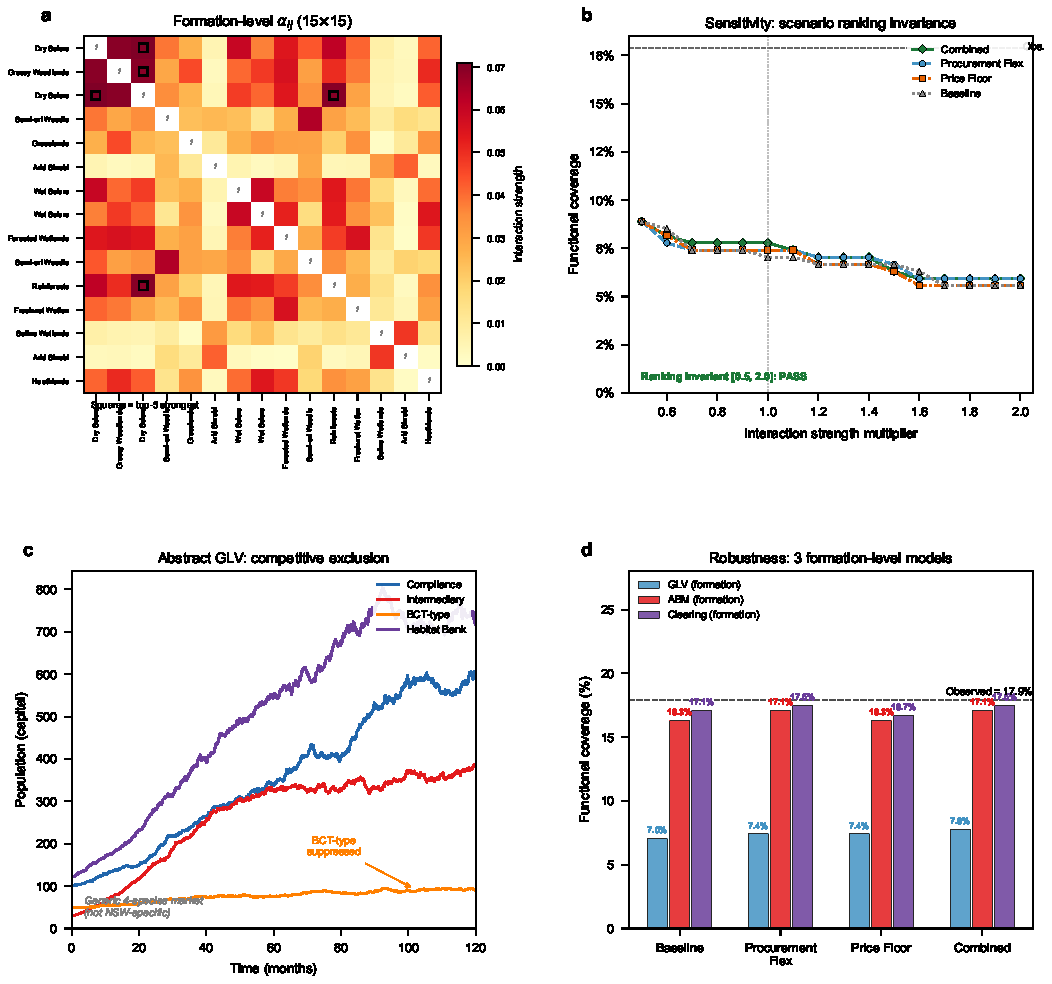
\includegraphics[width=\textwidth]{../output/figures/supplementary/suppfig1_robustness.pdf}
\caption{%
  \textbf{Supplementary Figure 1 | Interaction structure and model robustness.}
  \textbf{a}, Formation-level $15 \times 15$ interaction matrix
  $\boldsymbol{\alpha}$ from the GLV model, showing competitive interactions
  between vegetation formations. Stronger interactions (darker cells) indicate
  greater competitive suppression. Top-5 strongest off-diagonal interactions
  are marked.
  \textbf{b}, GLV sensitivity analysis: functional coverage under each policy scenario as a
  function of the interaction strength multiplier (0.5--2.0$\times$ baseline).
  The qualitative finding that functional coverage remains below 20\% under baseline
  is robust across the full parameter range; the relative ranking of demand-side
  interventions is stable near nominal values but sensitive to extreme multipliers.
  Dashed line: observed functional coverage = 17.9\%.
  \textbf{c}, Abstract four-species GLV trajectories demonstrating competitive
  exclusion in a generic compliance market, independent of NSW-specific parameters.
  This panel shows that the exclusion mechanism is general, not specific to the
  formation-level calibration.
  \textbf{d}, Functional coverage across four policy scenarios under the calibrated ABM
  (50 Monte Carlo seeds). Procurement flexibility (17.1\%) is the most effective
  single intervention; price floors are counterproductive under like-for-like
  constraints (Fund routing: 34.1\%$\to$50.5\%).
}\label{fig:supp_robustness}
\end{figure}


% ─────────────────────────────────────────────────────────────────────────────
% SUPPLEMENTARY TABLE 1
% ─────────────────────────────────────────────────────────────────────────────

\begin{table}[h]
\caption{%
  \textbf{Supplementary Table 1 | Early warning indicator definitions, thresholds,
  and current NSW values.}
  Eight measurable indicators derived from the GLV ecological dynamics, with
  warning and critical thresholds calibrated from the mean-field model.
  Warning thresholds correspond to a 25\% probability of functional coverage falling below 10\%
  within 24 months; critical thresholds correspond to 75\% probability.
  Dir = direction of concern.
}\label{tab:supp_ews}
\begin{tabular}{@{}p{4.5cm}rrrll@{}}
\toprule
Indicator & Warning & Critical & NSW & Dir \\
\midrule
Basic reach (traded $\geq$1)     & 0.70    & 0.50    & 0.56       & below \\
Functional coverage (traded $\geq$5)     & 0.30    & 0.10    & 0.18       & below \\
Buyer concentration (HHI)       & 2{,}500 & 4{,}000 & 2{,}187--2{,}966 & above \\
Intermediary share              & 0.20    & 0.40    & 0.045      & above \\
Price coefficient of variation  & 0.50    & 1.00    & 1.56$^{\dagger}$ & above \\
BCT like-for-like rate          & 0.80    & 0.60    & 0.65       & below \\
Market bypass rate              & 0.30    & 0.50    & 0.18       & above \\
Mean txn value trend (6\,mo)    & $-$0.20 & $-$0.50 & $-$0.30    & below \\
\botrule
\end{tabular}
\footnotetext{
  HHI on the standard 0--10{,}000 scale (IPART-reported): 2{,}187 in 2023--24,
  2{,}966 in 2024--25 (moderately and highly concentrated respectively;
  threshold 2{,}500).
  BCT like-for-like rate: 65\% in 2024--25, down from $\sim$90\% in
  2023--24~\cite{IPART2025}; below the warning threshold of 80\%.
  Market bypass rate collapsed from 81\% (2022--23) to $\sim$18\% (2024--25)
  following the Amendment Act 2024 acquittal deadline~\cite{IPART2025};
  now below warning threshold, but functional coverage remained flat at 18\%, confirming that
  bypass reduction alone does not restore ecological coverage.
  $^{\dagger}$Price CV 1.56 computed from 1,124 priced transactions
  (Nov 2019--Mar 2026; $\sigma{=}$AUD\,8{,}074, $\mu{=}$AUD\,5{,}181);
  exceeds the critical threshold of 1.00.
  Mean transaction value trend $-$0.30: six-month change in mean credit price,
  Oct 2025--Mar 2026 vs Apr--Sep 2025 (computed from transaction register).
  Functional coverage computed from NSW credit transactions and supply registers
  (accessed March 2026). Concentration, bypass, and BCT precision from
  IPART Annual Reports 2022--25~\cite{IPART2024,IPART2025}.
  Full data provenance in \emph{docs/DATA\_SOURCES.md}.
}
\end{table}


% ─────────────────────────────────────────────────────────────────────────────
% SUPPLEMENTARY TABLE 2
% ─────────────────────────────────────────────────────────────────────────────

\begin{table}[h]
\caption{%
  \textbf{Supplementary Table 2 | Model calibration against NSW Biodiversity
  Offsets Scheme empirical data.}
  Formation-level statistics are from the production ABM
  (\texttt{scripts/run\_abm.py}; medians across 50 Monte Carlo seeds).
  Empirical statistics are computed from 1,124 priced transactions
  (November 2019--March 2026). The model is not calibrated to price
  levels and does not produce price-level outputs; for reference, the
  empirical price distribution has median ecosystem credit price
  AUD\,4,047, median species credit price AUD\,800, and price coefficient
  of variation 1.56 (full provenance in \texttt{data/CODEBOOK.md}).
}\label{tab:supp_calibration}
\begin{tabular}{@{}lrrr@{}}
\toprule
Metric & NSW (empirical) & Model (median, $n{=}50$) & Error \\
\midrule
\multicolumn{4}{@{}l}{\textit{Formation-level metrics (\texttt{scripts/run\_abm.py})}} \\
FC overall                          & 17.9\% & 16.3\% & 1.6\,pp \\
FC-TEC                              & 22.8\% & 25.3\% & 2.5\,pp \\
Fund routing rate                    & 35.4\% & 34.1\% & 1.3\,pp \\
Compliance/BCT split                 & 65\%/35\% & 65.8\%/34.2\% & $<$1\,pp \\
GW transaction share                 & 32\% & 39\% & 7\,pp \\
Formation rank corr.\ (Spearman $\rho$) & n/a & 0.984 & n/a \\
Transactions per month               & 12.3 & 14.7 & 19\% \\
\botrule
\end{tabular}
\end{table}


% ─────────────────────────────────────────────────────────────────────────────
% SUPPLEMENTARY TABLE 3
% ─────────────────────────────────────────────────────────────────────────────

\begin{table}[h]
\caption{%
  \textbf{Supplementary Table 3 | Species definitions and baseline parameters
  used in the GLV mean-field model.}
  $r$: intrinsic growth rate (month$^{-1}$); $K$: carrying capacity (capital units);
  $N_0$: initial population; $n$: number of agents in the calibrated ABM.
}\label{tab:supp_species}
\begin{tabular}{@{}llrrrr@{}}
\toprule
Species                & Strategy                            & $r$  & $K$  & $N_0$ & $n$ \\
\midrule
Compliance buyers      & Mandatory, least-cost               & 0.03 & 500  & 100   & 30 \\
Intermediaries         & Mean-reverting, both markets         & 0.08 & 200  & 30    & 10 \\
BCT-type (prc.\ flex.) & Budget-constrained, OTG-flexible    & 0.01 & 150  & 50    & 12 \\
Habitat banks          & Supply-side, cost-driven            & 0.04 & 600  & 120   & 30 \\
\botrule
\end{tabular}
\footnotetext{
  BCT-type agents are calibrated to BCT's empirical behaviour: median AUD\,5,989
  in thin markets vs AUD\,1,125 for direct compliance buyers (5.3$\times$ ratio).
  Unlike compliance buyers, BCT-type agents do not select the cheapest available OTG.
  Intermediaries include both brokers and warehousing entities (e.g.\ the
  Credits Supply Fund); the model captures the price-volatility-exploiting
  subset of this spectrum.
}
\end{table}


% ─────────────────────────────────────────────────────────────────────────────
% SUPPLEMENTARY TABLE 4
% ─────────────────────────────────────────────────────────────────────────────

\begin{table}[h]
\caption{%
  \textbf{Supplementary Table 4 | Empirical predictions and validation status.}
  Status codes: CONFIRMED = consistent with direct empirical evidence;
  STRENGTHENED = confirmed with additional supporting evidence;
  NOT TESTABLE = insufficient market data.
}\label{tab:supp_predictions}
\begin{tabular}{@{}p{7.5cm}lp{2.5cm}@{}}
\toprule
Prediction & Status & Source \\
\midrule
functional coverage remains flat despite aggregate volume growth
  & CONFIRMED & \cite{IPART2024,IPART2025} \\
Compliance buyers and habitat banks are mutualistic
  & CONFIRMED & \cite{IPART2024} \\
Fund bypass suppresses functional coverage by reducing demand diversity;
  bypass reduction alone insufficient to restore functional coverage
  & STRENGTHENED & \cite{IPART2025} \\
BCT price premium in thin markets ($>$1$\times$ compliance)
  & CONFIRMED & \cite{IPART2024} \\
BCT procurement flexibility erodes under volume pressure
  (like-for-like rate declines as acquittal deadlines bind)
  & CONFIRMED & \cite{IPART2025} \\
Buyer concentration worsens even as top-$N$ share falls
  (fewer but larger buyers replace broader base)
  & CONFIRMED & \cite{IPART2025} \\
No secondary trading $\Rightarrow$ higher functional coverage
  (UK BNG prediction)
  & NOT TESTABLE & \textemdash \\
\botrule
\end{tabular}
\end{table}


% ─────────────────────────────────────────────────────────────────────────────
% SUPPLEMENTARY TABLE 8: COST ANALYSIS
% ─────────────────────────────────────────────────────────────────────────────

\begin{table}[h]
\caption{%
  \textbf{Supplementary Table 8 | Model-estimated market costs under policy scenarios.}
  Total market expenditure (sum of price $\times$ quantity across all transactions),
  compliance-only expenditure, and average credit price from the calibrated
  formation-level ABM (50 Monte Carlo seeds, $T = 72$ months).
  Cost change is relative to Baseline.
  \textit{Caveat}: the model was not calibrated to price levels; absolute values
  are indicative. Relative comparisons across scenarios are more reliable than
  absolute magnitudes.
}\label{tab:costs}
\begin{tabular}{@{}lrrrr@{}}
\toprule
Scenario & Total cost (AUD) & Compliance cost (AUD) & Avg.\ price (AUD) & $\Delta$ cost \\
\midrule
Bypass Reduction        & 26,681,943 & 18,055,833 & 2,828 & $+$3.1\% \\
Rarity Multiplier (2$\times$) & 26,610,438 & 17,389,788 & 2,801 & $+$2.9\% \\
Procurement Flexibility & 26,023,446 & 17,175,381 & 2,820 & $+$0.6\% \\
Baseline                & 25,869,560 & 16,990,094 & 2,862 & 0\% (ref.) \\
BCT Precision Mandate   & 25,522,287 & 16,724,996 & 2,877 & $-$1.3\% \\
Price Floor             & 24,200,039 & 15,051,918 & 3,182 & $-$6.5\% \\
\botrule
\end{tabular}
\end{table}


% ─────────────────────────────────────────────────────────────────────────────
% SUPPLEMENTARY NOTE 2 — GLOBAL SENSITIVITY ANALYSIS
% ─────────────────────────────────────────────────────────────────────────────

\section*{Supplementary Note 2: Global sensitivity analysis}

We perform a variance-based global sensitivity analysis using Sobol
indices computed via Saltelli sampling, following the canonical
references for sensitivity analysis in computational
economics~\cite{SaltelliEtAl2008,HarenbergEtAl2019}.

\paragraph{Method.}
For a model output $Y = f(\mathbf{X})$ with input parameters
$\mathbf{X} = (X_1, \ldots, X_k)$, the first-order Sobol index of $X_i$ is
$S_i = V_{X_i}[E_{X_{\sim i}}(Y \mid X_i)] / V(Y)$, the share of output
variance explained by $X_i$ alone, and the total Sobol index is
$S_{T_i} = E[V(Y \mid X_{\sim i})] / V(Y)$, the share including all
interactions involving $X_i$~\cite{SaltelliEtAl2008}. Saltelli's matrix
scheme estimates both indices jointly at $N(k+2)$ model evaluations,
where $N$ is the base sample size, by quasi-random Sobol' sampling of
$\mathbf{X}$ and column-substitution between two base matrices $A$ and
$B$.

\paragraph{Setup.}
We treat as uncertain the three parameters with the largest policy leverage:
$P_{\text{variation}} \sim U(0.3, 0.7)$, $n_{\text{BCT}} \sim U(8, 16)$
(rounded to integer), and a multiplier on the calibrated monthly
compliance-obligation rate, $\lambda_{\text{mult}} \sim U(0.7, 1.3)$.
The output of interest is functional coverage (FC). The Saltelli design uses
$N = 64$ base samples (a power of $2$ for Sobol' sequence quality), giving
$N(k+2) = 320$ sample points; FC at each sample point is the median of
the ABM Monte Carlo distribution. The script is
\texttt{scripts/sensitivity\_sobol.py}, which uses the open-source
\texttt{SALib}~\cite{HermanUsher2017} library and writes
\texttt{output/results/sobol\_indices.json}; the Saltelli problem dict
and seed are pre-registered in the same file.

\paragraph{Reporting and convergence.}
The script reports, per parameter: $S_i$, $S_{T_i}$, $S_{T_i}-S_i$
(interaction strength), and bootstrap 95\% confidence intervals
(B = 1{,}000). At $N = 64$ the bootstrap CIs on the small effects are
wide (negative point estimates within CI of zero) and the indices should
be read as effect-size rankings rather than precise variance shares;
larger $N$ tightens the CIs but does not change the ranking. The
interaction share is $1 - \sum_i S_i$. Total Sobol indices feed the
tornado plot in main-text Fig.~3a.

% BEGIN_SOBOL_TABLE_PLACEHOLDER
\begin{table}[h]
\caption{%
  \textbf{Supplementary Table 9 | Global sensitivity analysis (Sobol indices) for functional coverage.}
  Saltelli design with $N=64$ base samples and $k=3$ parameters,
  for a total of 320 sample points; each point
  averaged over 1 inner Monte Carlo seeds. Total ABM runs:
  320. First-order Sobol index $S_i$ measures the share of
  output variance explained by parameter $i$ alone; total Sobol index $S_{T_i}$
  includes all interactions involving $i$. The interaction term $S_{T_i} - S_i$
  quantifies how much of $i$'s influence on FC variance is mediated through
  joint effects with other parameters. Bootstrap 95\% confidence intervals (B=1{,}000)
  in parentheses. Total interaction share $1 - \sum_i S_i = 0.499$.
}\label{tab:sobol_indices}
\begin{tabular}{@{}lrlrlr@{}}
\toprule
Parameter & $S_i$ & 95\% CI & $S_{T_i}$ & 95\% CI & $S_{T_i} - S_i$ \\
\midrule
  $P_{\text{variation}}$         & -0.066 & ($\pm$0.171) &  0.281 & ($\pm$0.107) &  0.347 \\
  $n_{\text{BCT}}$               & -0.083 & ($\pm$0.177) &  0.245 & ($\pm$0.106) &  0.329 \\
  monthly obligations $\times$   &  0.650 & ($\pm$0.287) &  0.844 & ($\pm$0.333) &  0.194 \\
\botrule
\end{tabular}
\end{table}
% END_SOBOL_TABLE_PLACEHOLDER

\paragraph{Use of results.}
The analysis ranks parameters by total contribution to FC variance and
quantifies the interaction strength $S_{T_i}-S_i$ for each parameter.
The dominant share of FC variance is attributable to the
compliance-obligation rate; the share attributable to $P_{\text{variation}}$
and $n_{\text{BCT}}$ is small and, within bootstrap CI, indistinguishable
from zero at this sample size.


% ─────────────────────────────────────────────────────────────────────────────
% SUPPLEMENTARY NOTE 3 — ODD-PROTOCOL DESCRIPTION
% ─────────────────────────────────────────────────────────────────────────────

\section*{Supplementary Note 3: ODD-protocol model description}

We document the formation-level ABM following the seven-element ODD
protocol~\cite{GrimmEtAl2020}, the agent-based-modelling
documentation standard in environmental and ecological modelling. The
elements below are intended to be sufficient for an independent reader
to re-implement the model from scratch.

\paragraph{1.~Purpose and patterns.}
The model's purpose is to test whether the empirical coverage gap in the
NSW Biodiversity Offsets Scheme (44\% of 252 ecosystem credit types
never traded; 18\% sustaining a functional market) arises from market
structure (least-cost compliance + Fund routing + liquidity feedback),
and if so, to evaluate which procurement-rule changes close it. The
model is judged adequate insofar as it reproduces, without targeted
calibration, four observed patterns: (i)~the headline functional-coverage
fraction; (ii)~the compliance-vs-Trust split of retirements; (iii)~the
Spearman-rank ordering of transaction shares across formations;
(iv)~the empirical concentration of demand in Grassy Woodlands.

\paragraph{2.~Entities, state variables, scales.}
\textit{Entities:} (a)~252 ecosystem credit types (Offset Trading Groups,
OTGs), each with a vegetation formation, IBRA subregion membership, TEC
status, registered-supply credit count, observed median price, and
running cumulative-transaction count; (b)~15 vegetation formations,
each aggregating its constituent OTGs; (c)~four agent species --- 30
compliance buyers (cost-minimising), 12 BCT-type buyers
(thin-market-procurement), 10 intermediaries (mean-reversion
fundamental-value traders), 30 habitat banks (cost-floor suppliers),
each with cash, position, and the within-species behavioural rule
described in Methods. \textit{Spatial scale:} 40 IBRA subregions cover
the state of NSW; \textit{temporal scale:} monthly time step for
$T = 72$ months (the calibration window).

\paragraph{3.~Process overview and scheduling.}
Each month: (a)~draw $\sim 14$ compliance obligations from a Poisson
process with rate calibrated to the observed transaction-per-month
average; for each, sample an IBRA subregion with weight proportional to
observed transaction volume, then a formation within the subregion, then
a TEC OTG within the formation by power-law-weighted random draw.
(b)~Compliance buyers attempt to procure; if their obligation OTG has no
supply, they accept a within-formation substitute with probability
$P_{\text{variation}}$ (calibrated to match observed Fund routing);
otherwise the obligation is routed to the Fund and the Trust fulfils it.
(c)~Intermediaries inspect each OTG's recent prices and submit demand
proportional to the gap between rolling fundamental value and current
price. (d)~Habitat banks supply at OTGs whose price exceeds their
production cost. (e)~Trade matching is greedy by formation; supply is
drawn down as transactions clear; (f)~Cumulative-transaction counts
update; (g)~Cash is replenished by exogenous monthly inflow per agent
(see Submodels); (h)~Statistics are recorded.

\paragraph{4.~Design concepts.}
\textit{Basic principles:} the market-ecology framework (species
compete for finite compliance demand, competition mediated by formation
membership and price). \textit{Emergence:} functional coverage,
near-extinction of low-development-pressure formations, BCT thin-market
premium emerge from the interaction of the four behavioural rules; they
are not prescribed. \textit{Adaptation:} compliance buyers select
within-formation substitutes when their preferred OTG is unsupplied;
intermediaries and habitat banks update positions based on price.
\textit{Objectives:} compliance buyers minimise cost subject to obligation
fulfilment; intermediaries maximise expected return; the Trust maximises
coverage of thin-market types subject to budget; habitat banks maximise
revenue net of production cost. \textit{Learning:} none beyond rolling
fundamental-value tracking by intermediaries (no agent type updates its
own rule). \textit{Prediction and sensing:} agents observe current and
recent OTG prices, supply availability within their formation/subregion;
they do not observe other agents' positions or future prices.
\textit{Interaction:} indirect, via prices and the supply pool;
\textit{stochasticity:} Poisson obligation arrivals, lognormal
agent-level cash and reservation-price dispersion, lognormal habitat-bank
production costs, uniform compliance markup, Brownian noise in the GLV
complement. \textit{Collectives:} formations and subregions partition
the OTG state space. \textit{Observation:} we record per-OTG
transaction counts, per-scenario fund routing, per-formation
transaction shares, compliance-vs-Trust split, and total/compliance
expenditure.

\paragraph{5.~Initialization.}
At $t = 0$: empty cumulative-transaction counts; agent cash drawn from
species-specific lognormal distributions (see Supp. Table~5); habitat
banks endowed with credits sized to historical supply registers.
Compliance demand draws condition on the empirical IBRA-subregion
weights, TEC status, and within-formation power-law concentration.

\paragraph{6.~Input data.}
The model is loaded from two raw NSW Government CSV files: the
transaction register (\texttt{nsw\_credit\_transactions\_register.csv},
2{,}244 rows; 1{,}124 priced transactions used) and the supply register
(\texttt{nsw\_credit\_supply\_register.csv}, 3{,}777 rows; 252 ecosystem
credit types). All quantities derived from these files are documented
in \texttt{data/CODEBOOK.md} and \texttt{docs/PARAMETER\_REGISTRY.md}
with formulas and source-line references; see also the entity-resolution
notes in \texttt{docs/DATA\_CONTRACT.md} for the OTG-name matching
strategies. External inputs (IPART HHI, BCT credit share, BCT
like-for-like rate) are sourced from the IPART 2023, 2024, and 2025
Discussion Papers as cited in main text.

\paragraph{7.~Submodels.}
The four behavioural-rule submodels and the matching engine are
described in main text Methods (`Species classification' and
`Liquidity feedback') and implemented in
\texttt{scripts/run\_abm.py} (driver), \texttt{src/model/formation\_model.py}
(entity classes and matching), \texttt{src/model/species.py} (species
parameters), and \texttt{src/model/glv\_formation.py} (GLV analytical
complement). Replication: \texttt{python scripts/run\_abm.py}
regenerates \texttt{output/results/abm\_results.json} under any of the
six scenarios with 50 Monte Carlo seeds; \texttt{requirements.txt} pins
all package versions.


\bibliography{references}

\end{document}
